\documentclass{article}
\usepackage{ctex}
\usepackage[a4paper,left=10mm,right=10mm,top=15mm,bottom=15mm]{geometry}
\usepackage{graphicx}
\usepackage{amsfonts,amssymb}
\usepackage{amsmath}
\usepackage{biblatex}
\usepackage{hyperref}
\usepackage{color}
\usepackage{titlesec}
\usepackage{titletoc}

\title{VI-SLAM系统初始化闭式可解性分析}
\author{张谦}
\date{2020年3月13日}
\begin{document}
\maketitle
\tableofcontents
\newpage

\section{系统模型}
由VI-SLAM系统可观性分析可知,在给定视觉和IMU观测后,body系的全局平移和重力方向旋转yaw角不可观,
body系的速度、重力和绝对尺度是可观的。分析VI-SLAM系统初始化时的闭式可解性,亦即分析在一段时间内,
在不同条件下可观变量的可解性:(1)运动轨迹和状态;(2)地图点数量和观测图像上的分布;(3)相机图像帧数。

\subsection{几何关系}
为简化分析,不考虑相机和IMU之间的外参,即假设相机和IMU位姿重合。在该系统中,四元数表示旋转采用Hamilton形式。坐标系约定:全局坐标系用$G$表示,Camera坐标系用$C$表示,
IMU坐标系用$I$表示,地图点用$f$表示;相机、IMU和地图点表示在某个坐标系下,则该坐标系符号写在对应变量符号的左上角,
变量标识写在变量符号的右下角,例如$\sideset{^G}{}{\mathop{\mathbf{p}_{I}}}$表示IMU系(body系)原点在全局坐标系中的位置(平移),
$\sideset{^G}{}{\mathop{\textbf{v}_{I}}}$表示IMU系在全局坐标系下的速度,$\sideset{^G}{}{\mathop{\textbf{q}_{I}}}$表示从全局坐标系
旋转到IMU系的单位四元数,由于采用Hamilton形式,旋转均是由$I$系到$G$系旋转,与JPL表示方式相反;$\sideset{^G}{}{\mathop{\textbf{p}_{f_i}}}$
表示第$i$个地图点在$G$系下的坐标。
\begin{figure}[ht]
    \centering
    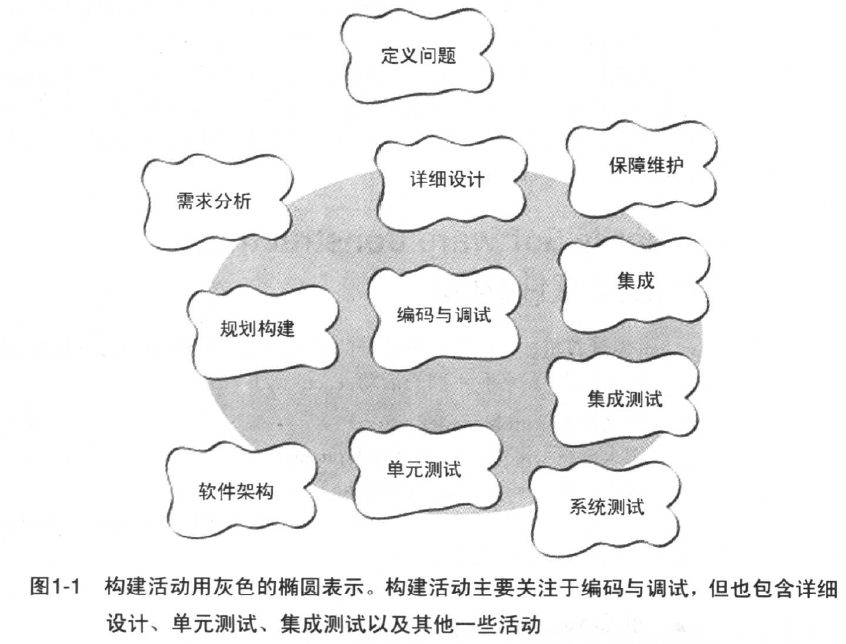
\includegraphics[width=15cm]{figure1.png}
    \caption{几何关系}
    \label{figs:geometryRelation}
\end{figure}

\par
陀螺仪测量$\sideset{^I}{}{\mathop{\mathbf{\omega}_m}}$和加速度计测量$\sideset{^I}{}{\mathop{\mathbf{a}_m}}$模型为:
\begin{equation}
    \sideset{^I}{}{\mathop{\mathbf{\omega}_{m}(t)}}=\sideset{^I}{}{\mathop{\mathbf{\omega}(t)}}
    +\textbf{b}_{g}(t)+\textbf{n}_{g}(t)
\end{equation}
\begin{equation}
    \sideset{^I}{}{\mathop{\mathbf{a}_{m}(t)}}=\textbf{C}^T(\sideset{^G}{}{\mathop{\mathbf{q}_{I}(t)}})
    (\sideset{^G}{}{\mathop{\mathbf{a}_{I}(t)}}-\sideset{^G}{}{\mathop{\mathbf{g}}})
    +\textbf{b}_{a}(t)+\textbf{n}_{a}(t)
\end{equation}
其中$\textbf{C}(\mathbf{q})$表示四元数对应的旋转矩阵。在分析可解性时,若不考虑噪声影响,则有,
\begin{equation}
    \sideset{^I}{}{\mathop{\mathbf{\omega}_{m}(t)}}=\sideset{^I}{}{\mathop{\mathbf{\omega}(t)}}
    +\textbf{b}_{g}(t)
\end{equation}
\begin{equation}
    \sideset{^G}{}{\mathop{\mathbf{a}_{I}(t)}}=\textbf{C}(\sideset{^G}{}{\mathop{\mathbf{q}_{I}(t)}})
    (\sideset{^I}{}{\mathop{\mathbf{a}_{m}(t)}}-\textbf{b}_{a}(t))
    +\sideset{^G}{}{\mathop{\mathbf{g}}}
\end{equation}

\par
现分析时间段$\left[t_{in},t_{fin}\right]$内的可解性,如图\ref{figs:geometryRelation}所示,
从$t_{in}$到$t\in\left[t_{in},t_{fin}\right]$时刻的平移几何关系可表示为,
\begin{equation}
    \begin{array}{ll}
        \sideset{^G}{}{\mathop{\textbf{p}_{I}}}(t)&=\sideset{^G}{}{\mathop{\textbf{p}_{I}}}(t_{in})+
        \sideset{^G}{}{\mathop{\textbf{v}_{I}}}(t_{in})\Delta{t}+\iint_{t_{in}}^{t}\sideset{^G}{}{\mathop{\mathbf{a}_{I}(\tau)}}d{\tau}^2\\
        &=\sideset{^G}{}{\mathop{\textbf{p}_{I}}}(t_{in})+
        \sideset{^G}{}{\mathop{\textbf{v}_{I}}}(t_{in})\Delta{t}+\iint_{t_{in}}^{t}
        (\textbf{C}(\sideset{^G}{}{\mathop{\mathbf{q}_{I}(\tau)}})(
        \sideset{^I}{}{\mathop{\mathbf{a}_{m}(\tau)}}-\textbf{b}_{a}(\tau))
        +\sideset{^G}{}{\mathop{\mathbf{g}}})d{\tau}^2\\
        &=\sideset{^G}{}{\mathop{\textbf{p}_{I}}}(t_{in})+
        \sideset{^G}{}{\mathop{\textbf{v}_{I}}}(t_{in})\Delta{t}
        +\frac{1}{2}\sideset{^G}{}{\mathop{\mathbf{g}}}\Delta{t}^{2}
        +\iint_{t_{in}}^{t}\textbf{C}(\sideset{^G}{}{\mathop{\mathbf{q}_{I}(\tau)}})
        (\sideset{^I}{}{\mathop{\mathbf{a}_{m}(\tau)}}-\textbf{b}_{a}(\tau))d{\tau}^2\\
        &=\sideset{^G}{}{\mathop{\textbf{p}_{I}}}(t_{in})+
        \sideset{^G}{}{\mathop{\textbf{v}_{I}}}(t_{in})\Delta{t}
        +\frac{1}{2}\sideset{^G}{}{\mathop{\mathbf{g}}}\Delta{t}^{2}
        +\textbf{C}(\sideset{^G}{}{\mathop{\mathbf{q}_{I}(t_{in})}})\textbf{C}^T(\sideset{^G}{}{\mathop{\mathbf{q}_{I}(t_{in})}})
        \iint_{t_{in}}^{t}\textbf{C}(\sideset{^G}{}{\mathop{\mathbf{q}_{I}(\tau)}})
        (\sideset{^I}{}{\mathop{\mathbf{a}_{m}(\tau)}}-\textbf{b}_{a}(\tau))d{\tau}^2\\
        &=\sideset{^G}{}{\mathop{\textbf{p}_{I}}}(t_{in})+
        \sideset{^G}{}{\mathop{\textbf{v}_{I}}}(t_{in})\Delta{t}
        +\frac{1}{2}\sideset{^G}{}{\mathop{\mathbf{g}}}\Delta{t}^{2}
        +\textbf{C}(\sideset{^G}{}{\mathop{\mathbf{q}_{I}(t_{in})}})
        \iint_{t_{in}}^{t}\textbf{C}^T(\sideset{^G}{}{\mathop{\mathbf{q}_{I}(t_{in})}})\textbf{C}(\sideset{^G}{}{\mathop{\mathbf{q}_{I}(\tau)}})
        (\sideset{^I}{}{\mathop{\mathbf{a}_{m}(\tau)}}-\textbf{b}_{a}(\tau))d{\tau}^2\\
        &=\sideset{^G}{}{\mathop{\textbf{p}_{I}}}(t_{in})+
        \sideset{^G}{}{\mathop{\textbf{v}_{I}}}(t_{in})\Delta{t}
        +\frac{1}{2}\sideset{^G}{}{\mathop{\mathbf{g}}}\Delta{t}^{2}
        +\textbf{C}(\sideset{^G}{}{\mathop{\mathbf{q}_{I}(t_{in})}})
        \iint_{t_{in}}^{t}\textbf{C}(\sideset{^{I_{in}}}{}{\mathop{\mathbf{q}_{I}(\tau)}})
        (\sideset{^I}{}{\mathop{\mathbf{a}_{m}(\tau)}}-\textbf{b}_{a}(\tau))d{\tau}^2\\
        &=\sideset{^G}{}{\mathop{\textbf{p}_{I}}}(t_{in})+
        \sideset{^G}{}{\mathop{\textbf{v}_{I}}}(t_{in})\Delta{t}
        +\frac{1}{2}\sideset{^G}{}{\mathop{\mathbf{g}}}\Delta{t}^{2}\\
        &\hspace{1cm}+\textbf{C}(\sideset{^G}{}{\mathop{\mathbf{q}_{I}(t_{in})}})
        (\iint_{t_{in}}^{t}\textbf{C}(\sideset{^{I_{in}}}{}{\mathop{\mathbf{q}_{I}(\tau)}})
        \sideset{^I}{}{\mathop{\mathbf{a}_{m}(\tau)}}d{\tau}^2
        -\iint_{t_{in}}^{t}\textbf{C}(\sideset{^{I_{in}}}{}{\mathop{\mathbf{q}_{I}(\tau)}})
        \textbf{b}_{a}(\tau)d{\tau}^2)
    \end{array}
\end{equation}
假设在积分区间内,加速度计bias为常量,则有,
\begin{equation}\label{eqs:imuInG}
    \begin{array}{ll}
        \sideset{^G}{}{\mathop{\textbf{p}_{I}}}(t)
        &=\sideset{^G}{}{\mathop{\textbf{p}_{I}}}(t_{in})+
        \sideset{^G}{}{\mathop{\textbf{v}_{I}}}(t_{in})\Delta{t}
        +\frac{1}{2}\sideset{^G}{}{\mathop{\mathbf{g}}}\Delta{t}^{2}\\
        &\hspace{1cm}+\textbf{C}(\sideset{^G}{}{\mathop{\mathbf{q}_{I}(t_{in})}})
        (\iint_{t_{in}}^{t}\textbf{C}(\sideset{^{I_{in}}}{}{\mathop{\mathbf{q}_{I}(\tau)}})
        \sideset{^I}{}{\mathop{\mathbf{a}_{m}(\tau)}}d{\tau}^2
        -\iint_{t_{in}}^{t}\textbf{C}(\sideset{^{I_{in}}}{}{\mathop{\mathbf{q}_{I}(\tau)}})
        d{\tau}^2\textbf{B})\\
        &=\sideset{^G}{}{\mathop{\textbf{p}_{I}}}(t_{in})+
        \sideset{^G}{}{\mathop{\textbf{v}_{I}}}(t_{in})\Delta{t}
        +\frac{1}{2}\sideset{^G}{}{\mathop{\mathbf{g}}}\Delta{t}^{2}
        +\textbf{C}(\sideset{^G}{}{\mathop{\mathbf{q}_{I}(t_{in})}})
        (\sideset{^{I_{in}}}{}{\mathop{\textbf{S}_{I}(t)}}
        -\sideset{^{I_{in}}}{}{\mathop{{\Gamma}_{I}(t)}}\textbf{B})
    \end{array}
\end{equation}
其中
\begin{equation}
    \sideset{^{I_{in}}}{}{\mathop{\textbf{S}_{I}(t)}}=\iint_{t_{in}}^{t}\textbf{C}(\sideset{^{I_{in}}}{}{\mathop{\mathbf{q}_{I}(\tau)}})
    \sideset{^I}{}{\mathop{\mathbf{a}_{m}(\tau)}}d{\tau}^2
\end{equation}
\begin{equation}\label{eqs:gammaDefine}
    \sideset{^{I_{in}}}{}{\mathop{{\Gamma}_{I}(t)}}=\iint_{t_{in}}^{t}\textbf{C}(\sideset{^{I_{in}}}{}{\mathop{\mathbf{q}_{I}(\tau)}})
    d{\tau}^2
\end{equation}
且$\sideset{^{I_{in}}}{}{\mathop{\textbf{S}_{I}(t)}}$和$\sideset{^{I_{in}}}{}{\mathop{{\Gamma}_{I}(t)}}$可由加速度计和陀螺仪提供的测量积分得到。

\par
现假设有N个地图点被同时观测到,$\sideset{^G}{}{\mathop{\textbf{p}_{f_i}}},i=1,\dots,N$,表示在第$t$时刻的相机
坐标系下为$\sideset{^{I_t}}{}{\mathop{\textbf{p}_{f_i}}}$,则有,
\begin{equation}\label{eqs:mappointInG1}
    \sideset{^G}{}{\mathop{\textbf{p}_{f_i}}}=\sideset{^G}{}{\mathop{\textbf{p}_I}}(t)
    +\textbf{C}(\sideset{^G}{}{\mathop{\textbf{q}_{I}}}(t_{in}))\textbf{C}(\sideset{^{I_{in}}}{}{\mathop{\textbf{q}_{I}}}(t))
    \sideset{^{I_t}}{}{\mathop{\textbf{p}_{f_i}}}
\end{equation}
若上式中$t=t_{in}$,则有,
\begin{equation}\label{eqs:mappointInG2}
    \sideset{^G}{}{\mathop{\textbf{p}_{f_i}}}=\sideset{^G}{}{\mathop{\textbf{p}_I}}(t_{in})
    +\textbf{C}(\sideset{^G}{}{\mathop{\textbf{q}_{I}}}(t_{in}))
    \sideset{^{I_{in}}}{}{\mathop{\textbf{p}_{f_i}}}
\end{equation}
将(\ref{eqs:imuInG})和(\ref{eqs:mappointInG2})带入(\ref{eqs:mappointInG1}),得到,
\begin{equation}
    \begin{array}{ll}
        \sideset{^G}{}{\mathop{\textbf{p}_I}}(t_{in})
        +\textbf{C}(\sideset{^G}{}{\mathop{\textbf{q}_{I}}}(t_{in}))
        \sideset{^{I_{in}}}{}{\mathop{\textbf{p}_{f_i}}}
        &=\sideset{^G}{}{\mathop{\textbf{p}_{I}}}(t_{in})+
        \sideset{^G}{}{\mathop{\textbf{v}_{I}}}(t_{in})\Delta{t}
        +\frac{1}{2}\sideset{^G}{}{\mathop{\mathbf{g}}}\Delta{t}^{2}
        +\textbf{C}(\sideset{^G}{}{\mathop{\mathbf{q}_{I}(t_{in})}})
        (\sideset{^{I_{in}}}{}{\mathop{\textbf{S}_{I}(t)}}
        -\sideset{^{I_{in}}}{}{\mathop{{\Gamma}_{I}(t)}}\textbf{B})\\
        &\hspace{1cm}+\textbf{C}(\sideset{^G}{}{\mathop{\textbf{q}_{I}}}(t_{in}))\textbf{C}(\sideset{^{I_{in}}}{}{\mathop{\textbf{q}_{I}}}(t))
        \sideset{^{I_t}}{}{\mathop{\textbf{p}_{f_i}}}\\
        \Leftrightarrow
        \textbf{C}(\sideset{^G}{}{\mathop{\textbf{q}_{I}}}(t_{in}))
        \sideset{^{I_{in}}}{}{\mathop{\textbf{p}_{f_i}}}
        &=\sideset{^G}{}{\mathop{\textbf{v}_{I}}}(t_{in})\Delta{t}
        +\frac{1}{2}\sideset{^G}{}{\mathop{\mathbf{g}}}\Delta{t}^{2}
        +\textbf{C}(\sideset{^G}{}{\mathop{\mathbf{q}_{I}(t_{in})}})
        (\sideset{^{I_{in}}}{}{\mathop{\textbf{S}_{I}(t)}}
        -\sideset{^{I_{in}}}{}{\mathop{{\Gamma}_{I}(t)}}\textbf{B})\\
        &\hspace{1cm}+\textbf{C}(\sideset{^G}{}{\mathop{\textbf{q}_{I}}}(t_{in}))\textbf{C}(\sideset{^{I_{in}}}{}{\mathop{\textbf{q}_{I}}}(t))
        \sideset{^{I_t}}{}{\mathop{\textbf{p}_{f_i}}}
    \end{array}
\end{equation}
两边同时乘以$\textbf{C}^T(\sideset{^G}{}{\mathop{\textbf{q}_{I}}}(t_{in}))$,得到,
\begin{equation}\label{eqs:geometryRelation1}
    \begin{array}{ll}
        &\sideset{^{I_{in}}}{}{\mathop{\textbf{p}_{f_i}}}
        =\textbf{C}^T(\sideset{^G}{}{\mathop{\textbf{q}_{I}}}(t_{in}))
        (\sideset{^G}{}{\mathop{\textbf{v}_{I}}}(t_{in})\Delta{t}
        +\frac{1}{2}\sideset{^G}{}{\mathop{\mathbf{g}}}\Delta{t}^{2}
        +\textbf{C}(\sideset{^G}{}{\mathop{\mathbf{q}_{I}(t_{in})}})
        (\sideset{^{I_{in}}}{}{\mathop{\textbf{S}_{I}(t)}}
        -\sideset{^{I_{in}}}{}{\mathop{{\Gamma}_{I}(t)}}\textbf{B}))
        +\textbf{C}(\sideset{^{I_{in}}}{}{\mathop{\textbf{q}_{I}}}(t))
        \sideset{^{I_t}}{}{\mathop{\textbf{p}_{f_i}}}\\
        &\Leftrightarrow
        \textbf{C}(\sideset{^{I_{in}}}{}{\mathop{\textbf{q}_{I}}}(t))
        \sideset{^{I_t}}{}{\mathop{\textbf{p}_{f_i}}}
        =\sideset{^{I_{in}}}{}{\mathop{\textbf{p}_{f_i}}}
        -\sideset{^{I_{in}}}{}{\mathop{\textbf{v}_I}}\Delta{t}
        -\frac{1}{2}\sideset{^{I_{in}}}{}{\mathop{\mathbf{g}}}\Delta{t}^{2}
        -\sideset{^{I_{in}}}{}{\mathop{\textbf{S}_{I}(t)}}
        +\sideset{^{I_{in}}}{}{\mathop{{\Gamma}_{I}(t)}}\textbf{B}
    \end{array}
\end{equation}
其中
\begin{equation}
    \sideset{^{I_{in}}}{}{\mathop{\textbf{v}_I}}
    =\textbf{C}^T(\sideset{^G}{}{\mathop{\textbf{q}_{I}}}(t_{in}))
    \sideset{^G}{}{\mathop{\textbf{v}_{I}}}(t_{in})
\end{equation}
\begin{equation}
    \sideset{^{I_{in}}}{}{\mathop{\mathbf{g}}}
    =\textbf{C}^T(\sideset{^G}{}{\mathop{\textbf{q}_{I}}}(t_{in}))
    \sideset{^G}{}{\mathop{\mathbf{g}}}
\end{equation}

\par
假设在时间段$t_{in},t_{fin}$内,共有$M$帧图像:$t_1=t_{in}<t_2<\dots<t_M=t_{fin}$,且$N$个地图点
均被这M帧图像观测到。为简化书写,利用如下简写:
\begin{equation}
    \begin{array}{ll}
        &\textbf{P}_j^i\triangleq\textbf{C}(\sideset{^{I_{in}}}{}{\mathop{\textbf{q}_{I}}}(t_j))
        \sideset{^{I_{t_j}}}{}{\mathop{\textbf{p}_{f_i}}}\\
        &\textbf{P}^i \triangleq \sideset{^{I_{in}}}{}{\mathop{\textbf{p}_{f_i}}}\\
        &\textbf{V} \triangleq \sideset{^{I_{in}}}{}{\mathop{\textbf{v}_I}}\\
        &\textbf{G} \triangleq \sideset{^{I_{in}}}{}{\mathop{\mathbf{g}}}\\
        &\Gamma_j \triangleq \sideset{^{I_{in}}}{}{\mathop{{\Gamma}_{I}(t_j)}}\\
        &\textbf{S}_j \triangleq \sideset{^{I_{in}}}{}{\mathop{\textbf{S}_{I}(t_j)}}
    \end{array}
\end{equation}
其中$i=1,2,\dots,N;\ \ j=1,2,\dots,M$。另外,用$\mathbf{\mu}_j^i$表示$\textbf{P}_j^i$的单位向量,
则有$\textbf{P}_j^i=\lambda_j^i\mathbf{\mu}_j^i$。不失一般性,可令$t_{in}=0$,则有$\Delta{t}=t$。
几何关系式(\ref{eqs:geometryRelation1})在每个图像帧时刻$t_j$,可表示为
\begin{equation}\label{eqs:geometryRelation2}
    \textbf{P}^i-\textbf{V}t_j-\frac{1}{2}\textbf{G}t_j^2+\Gamma_j\textbf{B}
    -\lambda_j^i\mathbf{\mu}_j^i=\textbf{S}_j
\end{equation}
另外当$j=1$时,$t_j=t_1=t_{in}=0$,则有$\textbf{P}^i=\textbf{P}^i_1=\lambda_1^i\mathbf{\mu}_1^i$。
几何关系(\ref{eqs:geometryRelation2})可进一步表示为,
\begin{equation}\label{eqs:geometryRelation3}
    -\textbf{V}t_j-\frac{1}{2}\textbf{G}t_j^2+\Gamma_j\textbf{B}+\lambda_1^i\mathbf{\mu}_1^i
    -\lambda_j^i\mathbf{\mu}_j^i=\textbf{S}_j
\end{equation}
对于第$t_1$帧和第$t_j$帧,第1个地图点和第$i$个地图点,有如下几何关系:
\begin{equation}\label{eqs:geometryRelation4}
    \lambda_1^1\mathbf{\mu}_1^1-\lambda_j^1\mathbf{\mu}_j^1
    =\lambda_1^i\mathbf{\mu}_1^i-\lambda_j^i\mathbf{\mu}_j^i
\end{equation}
综合几何关系(\ref{eqs:geometryRelation3})和(\ref{eqs:geometryRelation4}),可最终得到如下关系式子,
\begin{equation}\label{eqs:geometryRelation5}
    \left\{\begin{array}{c}
        -\textbf{V}t_j-\frac{1}{2}\textbf{G}t_j^2+\Gamma_j\textbf{B}+\lambda_1^1\mathbf{\mu}_1^1
        -\lambda_j^1\mathbf{\mu}_j^1=\textbf{S}_j\\
        \lambda_1^1\mathbf{\mu}_1^1-\lambda_j^1\mathbf{\mu}_j^1
        -\lambda_1^i\mathbf{\mu}_1^i+\lambda_j^i\mathbf{\mu}_j^i=\textbf{0}_3
    \end{array}\right.
\end{equation}
其中$j=2,3,\dots,M;\ \ i=2,3,\dots,N$。
分析VI-SLAM系统初始化的闭式可解性,亦即分析在几何关系(\ref{eqs:geometryRelation5})下,
变量$\textbf{P}^i_j,\textbf{V},\textbf{G},\textbf{B}$的可解性。其中(\ref{eqs:geometryRelation5})
可提供$3*(M-1)*N$个方程,未知变量有$M*N+6$维(不考虑bias)或$M*N+9$维(只考虑加速度计bias)。
\par
定义如下变量和矩阵:
考虑加速度计bias未知变量,
\begin{equation}
    \textbf{X}\triangleq\left[\textbf{G}^T,\textbf{V}^T,\textbf{B}^T,\lambda_1^1,\dots,\lambda_1^N,
    \dots,\lambda_M^1,\dots,\lambda_M^N\right]^T
\end{equation}
不考虑bias未知变量,
\begin{equation}
    \textbf{X}\triangleq\left[\textbf{G}^T,\textbf{V}^T,\lambda_1^1,\dots,\lambda_1^N,
    \dots,\lambda_M^1,\dots,\lambda_M^N\right]^T
\end{equation}
IMU测量相关积分变量,
\begin{equation}
    \textbf{S}\triangleq \left[\textbf{S}_2^T,\textbf{0}_{1\times3},\dots,\textbf{0}_{1\times 3},
    \textbf{S}_3^T,\textbf{0}_{1\times3},\dots,\textbf{0}_{1\times 3},
    \textbf{S}_M^T,\textbf{0}_{1\times3},\dots,\textbf{0}_{1\times 3}\right]^T
\end{equation}
几何关系矩阵,
\begin{equation}
    \Xi=\left[\begin{array}{cccccccccccccc}
        \textbf{T}_2&\textbf{K}_2&\Gamma_2&\mathbf{\mu}_1^1&\textbf{0}_{3\times 1}&\dots&\textbf{0}_{3\times 1}&
        -\mathbf{\mu}_2^1&\textbf{0}_{3\times 1}&\dots&\textbf{0}_{3\times 1}&\dots&\dots&\textbf{0}_{3\times 1}\\
        \textbf{0}_{3\times 3}&\textbf{0}_{3\times 3}&\textbf{0}_{3\times 3}&\mathbf{\mu}_1^1&-\mathbf{\mu}_1^2&\dots&\textbf{0}_{3\times 1}&
        -\mathbf{\mu}_2^1&\mathbf{\mu}_2^2&\dots&\textbf{0}_{3\times 1}&\dots&\dots&\textbf{0}_{3\times 1}\\
        \dots&\dots&\dots&\dots&\dots&\dots&\dots&\dots&\dots&\dots&\dots&\dots&\dots&\dots\\
        \textbf{0}_{3\times 3}&\textbf{0}_{3\times 3}&\textbf{0}_{3\times 3}&\mathbf{\mu}_1^1&\textbf{0}_{3\times 1}&\dots&-\mathbf{\mu}_1^N&
        -\mathbf{\mu}_2^1&\textbf{0}_{3\times 1}&\dots&\mathbf{\mu}_2^N&\dots&\dots&\textbf{0}_{3\times 1}\\
        \dots&\dots&\dots&\dots&\dots&\dots&\dots&\dots&\dots&\dots&\dots&\dots&\dots&\dots\\
        \dots&\dots&\dots&\dots&\dots&\dots&\dots&\dots&\dots&\dots&\dots&\dots&\dots&\dots\\
        \textbf{T}_M&\textbf{K}_M&\Gamma_M&\mathbf{\mu}_1^1&\textbf{0}_{3\times 1}&\dots&\dots&
        \dots&\dots&\dots&\textbf{0}_{3\times 1}&-\mathbf{\mu}_M^1&\dots&\textbf{0}_{3\times 1}\\
        \textbf{0}_{3\times 3}&\textbf{0}_{3\times 3}&\textbf{0}_{3\times 3}&\mathbf{\mu}_1^1&-\mathbf{\mu}_1^2&\dots&\dots&
        \dots&\dots&\dots&\textbf{0}_{3\times 1}&-\mathbf{\mu}_M^1&\mathbf{\mu}_M^2&\textbf{0}_{3\times 1}\\
        \dots&\dots&\dots&\dots&\dots&\dots&\dots&\dots&\dots&\dots&\dots&\dots&\dots&\dots\\
        \textbf{0}_{3\times 3}&\textbf{0}_{3\times 3}&\textbf{0}_{3\times 3}&\mathbf{\mu}_1^1&\textbf{0}_{3\times 1}&\dots&-\mathbf{\mu}_1^N&
        \textbf{0}_{3\times 1}&\dots&\dots&\textbf{0}_{3\times 1}&-\mathbf{\mu}_M^1&\dots&\mathbf{\mu}_M^N
    \end{array}\right]
\end{equation}
其中$\textbf{T}_j\triangleq -\frac{t_j^2}{2}\textbf{I}_3$和$\textbf{K}_j\triangleq -t_j\textbf{I}_3$。

\par
根据以上定义,对于M帧图像和N个地图点的几何关系式(\ref{eqs:geometryRelation5})可表示为
\begin{equation}\label{eqs:geometryRelation6}
    \Xi\textbf{X}=\textbf{S}
\end{equation}
假设重力的大小已知,即$|\textbf{G}|=g$,则对方程组(\ref{eqs:geometryRelation6})添加如下约束,
\begin{equation}\label{eqs:geometryRelation7}
    |\Pi\textbf{X}|^2=g^2
\end{equation}
其中$\Pi\triangleq \left[\textbf{I}_3,\textbf{0}_3,\dots,\textbf{0}_3\right]$。

\par
至此,VI-SLAM系统初始化的闭式可解性分析,将基于方程组(\ref{eqs:geometryRelation6})和(\ref{eqs:geometryRelation7})。
通过分析矩阵$\Xi$的零空间$\mathcal{N}(\Xi)$,可得到变量$\textbf{X}$的可解情况。

\subsection{基本原理}
关于VI-SLAM系统解的个数,有如下结论:
\par
\textbf{Theorem1:} (a)当矩阵$\Xi$的零空间$\mathcal{N}(\Xi)$为空时,有且仅有1个解;
(b)当零空间$dim(\mathcal{N}(\Xi))=1$,且对于任意$\textbf{n}\in\mathcal{N}(\Xi),\ \ |\Pi\textbf{n}|\not=0$时,
有2个解;(c)其他情况,有无数解。
\par
证明如下:$(\romannumeral1)$对于结论(a),显然地利用高斯消元法解方程组,可得到唯一解;$(\romannumeral2)$当$dim(\mathcal{N}(\Xi))=1$时,
线性方程组(\ref{eqs:geometryRelation6})有解:$\textbf{X}(\gamma)=\Xi^{-1}\textbf{S}+\gamma\textbf{n}$(左右乘以$\Xi$可验证),
其中$\Xi^{-1}$为$\Xi$的伪逆,$\textbf{n}$为零空间$\mathcal{N}(\Xi)$的列向量,$\gamma\in\mathbb{R}$为一个未知标量。
$\gamma$可由式子(\ref{eqs:geometryRelation7})解得:当$|\Pi\textbf{n}|\not=0$时,$|\Pi\textbf{X}(\gamma)|^2=g^2$
是关于$\gamma$的二次多项式,因此有两个解$\gamma_1$和$\gamma_2$,对应有两个解$\textbf{X}$,$\textbf{X}_1\triangleq \textbf{X}(\gamma_1)$
和$\textbf{X}_2\triangleq \textbf{X}(\gamma_2)$;当$|\Pi\textbf{n}|=0$时,$|\Pi\textbf{X}(\gamma)|^2=g^2$与$\gamma$不相关,因此有无数解,
但此时重力$\textbf{G}$可被唯一解出。

\par
结合\textbf{Theorem1}可通过分析矩阵$\Xi$的零空间$\mathcal{N}(\Xi)$,得到VI-SLAM系统的可解的情况。
由于矩阵的每一列乘以一个非零的标量常数,不改变矩阵零空间,为便于分析,将矩阵$\Xi$做如下变形,
亦即每一列乘以对应的$\lambda_j^i$还原为$\textbf{P}_j^i=\lambda_j^i\mathbf{\mu}_j^i$,得到
\begin{equation}
    \Xi'\triangleq \left[\begin{array}{cccccc}
        \mathcal{M}_2&\mathcal{P}_1&\mathcal{P}_2&\textbf{0}_{3N\times N}&\dots&\textbf{0}_{3N\times N}\\
        \mathcal{M}_3&\mathcal{P}_1&\textbf{0}_{3N\times N}&\mathcal{P}_3&\dots&\textbf{0}_{3N\times N}\\
        \dots&\dots&\dots&\dots&\dots&\dots\\
        \mathcal{M}_M&\mathcal{P}_1&\textbf{0}_{3N\times N}&\textbf{0}_{3N\times N}&\dots&\mathcal{P}_M
    \end{array}\right]
\end{equation}
其中
\begin{equation}
    \mathcal{M}_j\triangleq \left[\begin{array}{ccc}
        \textbf{T}_j&\textbf{K}_j&\Gamma_j\\
        \textbf{0}_{3\times 3}&\textbf{0}_{3\times 3}&\textbf{0}_{3\times 3}\\
        \dots&\dots&\dots\\
        \textbf{0}_{3\times 3}&\textbf{0}_{3\times 3}&\textbf{0}_{3\times 3}
    \end{array}\right]
\end{equation}
\begin{equation}
    \mathcal{P}_j\triangleq \left[\begin{array}{ccccc}
        \textbf{P}_j^1&\textbf{0}_{3\times 1}&\textbf{0}_{3\times 1}&\dots&\textbf{0}_{3\times 1}\\
        \textbf{P}_j^1&\textbf{P}_j^2&\textbf{0}_{3\times 1}&\dots&\textbf{0}_{3\times 1}\\
        \textbf{P}_j^1&\textbf{0}_{3\times 1}&\textbf{P}_j^3&\dots&\textbf{0}_{3\times 1}\\
        \dots&\dots&\dots&\dots&\dots\\
        \textbf{P}_j^1&\textbf{0}_{3\times 1}&\dots&\textbf{0}_{3\times 1}&\textbf{P}_j^N
    \end{array}\right]
\end{equation}
由式子(\ref{eqs:geometryRelation4})可知$\textbf{P}_j^i-\textbf{P}_1^i,i=1,2,\dots,N$独立于$i$,
因此令$\mathcal{X}_j\triangleq \textbf{P}_j^i-\textbf{P}_1^i$表征IMU系的运动状态。
为保证矩阵$\Xi'$的每一列不为零,做如下假设:
\par
\textbf{Assumption1:}对于任意$i=1,2,\dots,N,\ \ j=2,\dots,M$,有$\textbf{P}_j^i\not=\textbf{0}_{3\times 1}$。

\par
接下来,基于上述结论,通过分析矩阵$\Xi'$的零空间,进而分析考虑bias和不考虑bias时,VI-SLAM系统的可解性。

\section{可解性分析:Unbiased Case}
假设向量$\textbf{n}\in\mathcal{N}(\Xi')$,
\begin{equation}
    \textbf{n}\triangleq \left[\mathbf{\alpha}^T,\mathbf{\nu}^T,n_1^1,\dots,n_1^N,
    n_2^1,\dots,n_2^N,\dots,n_M^1,\dots,n_M^N\right]^T
\end{equation}
且有
\begin{equation}\label{eqs:geometryRelation8}
    \Xi'\textbf{n}=\textbf{0}_{3(M-1)*N\times 1}
\end{equation}
将上式展开得到
\begin{equation}\label{eqs:geometryRelation8_1}
    -\frac{1}{2}\mathbf{\alpha}t_j^2-t_j\mathbf{\nu}+(n_1^1+n_j^1)\textbf{P}_1^1+n_j^1\mathcal{X}_j=\textbf{0}_{3\times 1}
\end{equation}
\begin{equation}\label{eqs:geometryRelation8_2}
    (n_1^1+n_j^1)\textbf{P}_1^1+(n_1^i+n_j^i)\textbf{P}_1^i+(n_j^1+n_j^i)\mathcal{X}_j=\textbf{0}_{3\times 1}
\end{equation}
上面两个式子可通过如下方式验证成立:由式子(\ref{eqs:geometryRelation8_2})可知,
\begin{equation}
    \begin{array}{ll}
    (n_1^1+n_j^1)\textbf{P}_1^1+n_j^1\mathcal{X}_j
    &=-(n_1^i+n_j^i)\textbf{P}_1^i-n_j^i\mathcal{X}_j\\
    &=-(n_1^i+n_j^i)\textbf{P}_1^i-n_j^i(\textbf{P}_j^i-\textbf{P}_1^i)\\
    &=-n_1^i\textbf{P}_1^i-n_j^i\textbf{P}_1^i-n_j^i\textbf{P}_j^i+n_j^i\textbf{P}_1^i\\
    &=-n_1^i\textbf{P}_1^i-n_j^i\textbf{P}_j^i
    \end{array}
\end{equation}
由于$\mathcal{X}_j=\textbf{P}_j^i-\textbf{P}_1^i=\textbf{P}_j^1-\textbf{P}_1^1$,因此左式可写为,
\begin{equation}
    \begin{array}{ll}
    (n_1^1+n_j^1)\textbf{P}_1^1+n_j^1\mathcal{X}_j
    &=(n_1^1+n_j^1)\textbf{P}_1^1+n_j^1(\textbf{P}_j^1-\textbf{P}_1^1)\\
    &=n_1^1\textbf{P}_1^1+n_j^1\textbf{P}_j^1
    \end{array}
\end{equation}
即有,
\begin{equation}
    \begin{array}{c}
    n_1^1\textbf{P}_1^1+n_j^1\textbf{P}_j^1=-n_1^i\textbf{P}_1^i-n_j^i\textbf{P}_j^i\\
    \Leftrightarrow
    n_1^1\textbf{P}_1^1+n_j^1\textbf{P}_j^1+n_1^i\textbf{P}_1^i+n_j^i\textbf{P}_j^i=0
    \end{array}
\end{equation}

下面首先分析2D下共面和共线特殊情况,然后再分析3D下各种图像帧数和地图点数量的可解情况。
\subsection{Planar Case}
假设所有地图点和相机运动轨迹处在同一平面上,亦即$\textbf{P}_j^i,i=1,\dots,N,j=2,\dots,M$在同一平面上。
则矩阵$\Xi'$中所有$\textbf{P}_j^i$的某一维可以高斯消元为零:假设所有地图点和相机运动轨迹所在的同一平面
方程为$Ax+By+Cz+D=0$则$x,y,z$的其中之一可由另外两个变量线性表示。现假设在共面情况下,所有$\textbf{P}_j^i$
的第三维为零。注意变量$\mathbf{\alpha}$和$\mathbf{\nu}$的第三维不为零,因为公共平面可能为三维空间中的斜平面。
为方便分析,将系统(\ref{eqs:geometryRelation8})分为两部分:第一部分为(\ref{eqs:geometryRelation8_1})
和(\ref{eqs:geometryRelation8_2})的第一行和第二行组成的矩阵$\Xi_1^{plane}$,其维度为{\color{red}{$2(M-1)N\times (MN+4)$}};
第二部分为(\ref{eqs:geometryRelation8_1})的第三行组成的矩阵$\Xi_2^{plane}$,其只包含$\mathbf{\alpha}$和
$\mathbf{\nu}$的第三维,维度为{\color{red}{$(M-1)\times 2$}}。
\par
根据\textbf{Theorem1},
\par
(1)当$M\leqslant 2$时,$dim(\mathcal{N}(\Xi_1^{plane}))\geqslant 4$;保证系统具有
有限个解的先决条件为$M\geqslant 3$。
\par
(2)当$M\geqslant 3$时,$dim(\mathcal{N}(\Xi_2^{plane}))=0$;
\par
(3)当$M=3$时,矩阵$\Xi_1^{plane}$的维度为$4N\times (3N+4)$;因此为了使$dim(\mathcal{N}(\Xi_1^{plane}))\leqslant 1$,
至少需要保证$N\geqslant 3$;
\par
(4)当$M=4$时,矩阵$\Xi_1^{plane}$的维度为$6N\times (4N+4)$;因此为了使$dim(\mathcal{N}(\Xi_1^{plane}))\leqslant 1$,
至少需要保证$N\geqslant 2$;
\par
(5)当$M\geqslant 5$时,$N$无要求。

\subsection{Linear Case}
假设所有地图点和相机运动轨迹共线,亦即$\textbf{P}_j^i,i=1,\dots,N,j=2,\dots,M$在同一条线上。则矩阵$\Xi'$中
所有$\textbf{P}_j^i$的某两维可以高斯消元为零:根据空间直线方程,$\textbf{P}_j^i$任意一维可线性表示另外两维。
现假设在共线情况下,所有$\textbf{P}_j^i$的第二、三维为零。同样的,为方便分析,
将系统(\ref{eqs:geometryRelation8})分为两部分:第一部分为(\ref{eqs:geometryRelation8_1})
和(\ref{eqs:geometryRelation8_2})的第一行组成的矩阵$\Xi_1^{line}$,其维度为{\color{red}{$(M-1)N\times (MN+2)$}};
第二部分为(\ref{eqs:geometryRelation8_1})的第二、三行组成的矩阵$\Xi_2^{line}$,其只包含$\mathbf{\alpha}$和
$\mathbf{\nu}$的第二、三维,维度为{\color{red}{$2(M-1)\times 4$}}。显然地,$dim(\mathcal{N}(\Xi_1^{line})>2$,
根据\textbf{Theorem1},系统在任何条件下,均有无数解。

\newpage
接下来,讨论一般3D情况下的系统可解性。首先给出性质:
\par
\textbf{Property1: } (a)当$M\leqslant 2$时,$dim(\mathcal{N}(\Xi'))\geqslant 3$;
(b)当$M=3$时,$dim(\mathcal{N}(\Xi'))\geqslant 1$;
(c)当$M\geqslant 4$,且相机匀加速运动时,$dim(\mathcal{N}(\Xi'))\geqslant 1$。
\par
证明如下:首先定义一个子系统,
\begin{equation}\label{eqs:geometryRelation9}
    -\frac{1}{2}\mathbf{\alpha}t_j^2-t_j\mathbf{\nu}=-\mathcal{X}_j, j=2,\dots,M
\end{equation}
且由其构成的方程组矩阵为$\Xi''$,维度为{\color{red}{$3(M-1)\times 6$}}。显然的,$dim(\mathcal{N}(\Xi''))\leqslant dim(\mathcal{N}(\Xi'))$。
假如变量$\left[\textbf{n}_\mathbf{\alpha}^T,\textbf{n}_\mathbf{\nu}^T\right]^T\in\mathcal{N}(\Xi'')$,
则由$\mathbf{\alpha}=\textbf{n}_{\mathbf{\alpha}},\mathbf{\nu}=\textbf{n}_{\mathbf{\nu}},n_j^i=0, \forall i,j$
组成的向量$\textbf{n}\in \mathcal{N}(\Xi')$。
\par
(1)当$M\leqslant 2$时,$dim(\mathcal{N}(\Xi''))\geqslant 3$;
\par
(2)当$M=3$时,矩阵$\Xi''$的维度为$6\times 6$,方程组(\ref{eqs:geometryRelation9})有唯一解$(\mathbf{\alpha}_0,\mathbf{\nu}_0)$;
对应的,矩阵$\Xi'$由如下零空间,
\begin{equation}\label{eqs:zeroSpace}
    \textbf{n}_0\triangleq \left[\mathbf{\alpha}_0^T,\mathbf{\nu}_0^T,\bar{n}_1^1,\dots,\bar{n}_1^i,
    \dots,\bar{n}_j^1,\dots,\bar{n}_j^i,\dots\right]^T
\end{equation}
其中$\bar{n}_1^1=-1,\bar{n}_j^1=1,\bar{n}_1^i=1,\bar{n}_j^i=-1;\ j=2,3;\ i=2,3,\dots,N$。
即当$M=3$时,$\textbf{n}_0\in \mathcal{N}(\Xi')$,则$dim(\mathcal{N}(\Xi'))\geqslant 1$
\par
(3)当$M\geqslant 4$时,系统(\ref{eqs:geometryRelation9})有解条件为:
当且仅当$\mathcal{X}_j=\mathbf{\nu}_{0}t_{j}+\frac{1}{2}\mathbf{\alpha}_0t_j^2$,
亦即对每个$j$,均有$\mathbf{\alpha}=\mathbf{\alpha}_0, \mathbf{\nu}=\mathbf{\nu}_0$。
此时矩阵$\Xi''$有零空间$\left[\mathbf{\alpha}_0^T,\mathbf{\nu}_0^T\right]^T$,
进而矩阵$\Xi'$有零空间$\textbf{n}_0$,即$\textbf{n}_0\in \mathcal{N}(\Xi')$,
对应相机以初速度$\mathbf{\nu}_0$做加速度为$\mathbf{\alpha}_0$的匀加速运动。

\par
根据\textbf{Theorem1},为分析系统的有限解情况,需要分析$\textbf{n}_0$是否为矩阵$\Xi'$的唯一零空间向量。
接下来分不同情况考虑分析。

\subsection{图像帧数小于等于2}
根据\textbf{Property1},$dim(\mathcal{N}(\Xi'))\geqslant 3$;由\textbf{Theorem1}可知,系统有无限个解。

\subsection{图像帧数等于3}
根据\textbf{Property1},$dim(\mathcal{N}(\Xi'))\geqslant 1$。
\par
(1)当$N=1$时,矩阵$\Xi'$的维度为$6\times 9$,因此$dim(\mathcal{N}(\Xi'))\geqslant 3$,系统有无限解。
\par
(2)当$N=2$时,矩阵$\Xi'$的维度为$12\times 12$。当且仅当如下两个条件满足时,$dim(\mathcal{N}(\Xi'))=1$:
(\romannumeral1)对于给定的$j$(例如$j=2$或$j=3$),三个向量$\textbf{P}_1^1,\textbf{P}_1^2,\mathcal{X}_j$
生成3D空间,即三个向量不在同一平面上;
(\romannumeral2)对于其他的$j$(例如$j=3$或$j=2$),$\textbf{P}_j^i$与$\textbf{P}_j^k,\forall i,k=1,2,\dots,N$
不成比例,即不共线。否则,$dim(\mathcal{N}(\Xi'))\geqslant 1$。
\par
证明如下:当(\romannumeral1)不满足时,即三个向量$\textbf{P}_1^1,\textbf{P}_1^2,\mathcal{X}_j$共面;
由于$N=2$,根据上面Planar Case的讨论,$dim(\mathcal{N}(\Xi'))>1$。现假设条件(\romannumeral1)对于给定的
$j=2$成立,依据公式(\ref{eqs:geometryRelation8_2}),由于三个向量不共面,即任意一个向量不能被另外两个向量线性表示,
为使等式成立,则三个向量前的系数为零,可得$n_1^1=n_2^2=-n_2^1=-n_1^2$。
根据公式(\ref{eqs:geometryRelation8_1}),当$j=2$时,
可得$-\frac{1}{2}\mathbf{\alpha}t_2^2-t_2\mathbf{\nu}=-n_2^1\mathcal{X}_2$,与系统(\ref{eqs:geometryRelation9})
类似(用$n_2^1\mathcal{X}_2$代替$\mathcal{X}_2$)。依据公式(\ref{eqs:geometryRelation8_2}),当$j=3$时,取$i=2$,
\begin{equation}
    \begin{array}{ll}
        &\hspace{0.5cm}(n_1^1+n_3^1)\textbf{P}_1^1+(n_1^2+n_3^2)\textbf{P}_1^2+(n_3^1+n_3^2)\mathcal{X}_3=\textbf{0}_{3\times 1}\\
        &\Leftrightarrow
        (n_1^1+n_3^1)\textbf{P}_1^1+(n_1^2+n_3^2)\textbf{P}_1^2+(n_1^1+n_3^1+n_1^2+n_3^2)\mathcal{X}_3=\textbf{0}_{3\times 1}\\
        &\Leftrightarrow
        (n_1^1+n_3^1)(\textbf{P}_1^1+\mathcal{X}_3)+(n_1^2+n_3^2)(\textbf{P}_1^2+\mathcal{X}_3)=\textbf{0}_{3\times 1}\\
        &\Leftrightarrow
        (n_1^1+n_3^1)\textbf{P}_3^1+(n_1^2+n_3^2)\textbf{P}_3^2=\textbf{0}_{3\times 1}\\
        &\Leftrightarrow
        (-n_2^1+n_3^1)\textbf{P}_3^1=-(n_2^1+n_3^2)\textbf{P}_3^2
    \end{array}
\end{equation}
其中利用了$n_1^1=-n_2^1=-n_1^2$和$\mathcal{X}_3=\textbf{P}_3^1-\textbf{P}_1^1=\textbf{P}_3^2-\textbf{P}_1^2$。
当条件(\romannumeral2)成立时,有$\textbf{P}_3^1$和$\textbf{P}_3^2$不共线,则它们前面的系数为零,得到
$n_3^1=-n_3^2=n_2^1$。
根据公式(\ref{eqs:geometryRelation8_1}),当$j=3$时,
可得$-\frac{1}{2}\mathbf{\alpha}t_3^2-t_3\mathbf{\nu}=-n_3^1\mathcal{X}_3=-n_2^1\mathcal{X}_3$,
与系统(\ref{eqs:geometryRelation9})类似(用$n_2^1\mathcal{X}_3$代替$\mathcal{X}_3$)。
至此,当$j=2,3$且满足条件(\romannumeral1)和(\romannumeral2)时,系统与(\ref{eqs:geometryRelation9})类似,
仅仅用$n_2^1\mathcal{X}_j$代替$\mathcal{X}_j$;根据上面讨论,该系统有唯一解,且零空间$\mathcal{N}(\Xi')$
仅有生成向量$\textbf{n}_0$。根据\textbf{Theorem1},系统有2个解。
\par
综上所述,当$M=3,N\geqslant 2$时,满足相关条件时,VI-SLAM系统有2个解;否则有无数个解。


\subsection{图像帧数大于等于4}
当$M\geqslant 4$时,方程个数大于未知数个数;除了当$M=4,N=1$时,矩阵$\Xi'$的维度为$9\times 10$,
其零空间维度至少为1维。下面首先分析该特殊情况。
\par
(1)当$M=4,N=1$时,当且仅当4个向量$\textbf{P}_1^1,\mathcal{X}_2,\mathcal{X}_3,\mathcal{X}_4$
生成整个3D空间,即该4个向量不共面时,$dim(\mathcal{N}(\Xi'))=1$。
\par
证明如下:假如4个向量共面,根据Planar Case的讨论,由于$N=1$,$dim(\mathcal{N}(\Xi'))>1$。
下面考虑4个向量不共面,且生成3D空间的情况。根据公式(\ref{eqs:geometryRelation8}),首先取前6个方程,
即公式(\ref{eqs:geometryRelation8_1})中$j=2,3$,可得到$\mathbf{\alpha}$和$\mathbf{\nu}$关于
$\textbf{P}_1^1,\mathcal{X}_2,\mathcal{X}_3$的线性表示:
\begin{equation}\label{eqs:j23}
    \begin{array}{c}
    \left\{\begin{array}{c}
        -\frac{1}{2}\mathbf{\alpha}t_2^2-t_2\mathbf{\nu}+(n_1^1+n_2^1)\textbf{P}_1^1+n_2^1\mathcal{X}_2=\textbf{0}_{3\times 1}\\
        -\frac{1}{2}\mathbf{\alpha}t_3^2-t_3\mathbf{\nu}+(n_1^1+n_3^1)\textbf{P}_1^1+n_3^1\mathcal{X}_3=\textbf{0}_{3\times 1}
    \end{array}\right.\\
    \Leftrightarrow
    \left\{
    \begin{array}{c}
        \mathbf{\alpha}=\frac{2}{t_{3}t_2^2-t_{2}t_3^2}
        \left\{\left[t_{3}(n_1^1+n_2^1)-t_{2}(n_1^1+n_3^1)\right]\textbf{P}_1^1
        +t_{3}n_2^1\mathcal{X}_2-t_{2}n_3^1\mathcal{X}_3\right\}\\
        \mathbf{\nu}=\frac{1}{t_{2}t_3^2-t_{3}t_2^2}
        \left\{\left[t_{3}^{2}(n_1^1+n_2^1)-t_{2}^{2}(n_1^1+n_3^1)\right]\textbf{P}_1^1
        +t_{3}^{2}n_2^1\mathcal{X}_2-t_{2}^{2}n_3^1\mathcal{X}_3\right\}
    \end{array}\right.
    \end{array}
\end{equation}
将$\mathbf{\alpha}$和$\mathbf{\nu}$带入到$j=4$的公式(\ref{eqs:geometryRelation8_1})中,得到
\begin{equation}\label{eqs:j234}
    \begin{array}{c}
        -\frac{1}{2}\mathbf{\alpha}t_4^2-t_4\mathbf{\nu}+(n_1^1+n_4^1)\textbf{P}_1^1+n_4^1\mathcal{X}_4=\textbf{0}_{3\times 1}\\
        \Leftrightarrow
        -\frac{t_4^2}{t_{3}t_2^2-t_{2}t_3^2}
        \left\{\left[t_{3}(n_1^1+n_2^1)-t_{2}(n_1^1+n_3^1)\right]\textbf{P}_1^1
        +t_{3}n_2^1\mathcal{X}_2-t_{2}n_3^1\mathcal{X}_3\right\}\\
        -\frac{t_4}{t_{2}t_3^2-t_{3}t_2^2}
        \left\{\left[t_{3}^{2}(n_1^1+n_2^1)-t_{2}^{2}(n_1^1+n_3^1)\right]\textbf{P}_1^1
        +t_{3}^{2}n_2^1\mathcal{X}_2-t_{2}^{2}n_3^1\mathcal{X}_3\right\}
        +(n_1^1+n_4^1)\textbf{P}_1^1+n_4^1\mathcal{X}_4=\textbf{0}_{3\times 1}
    \end{array}
\end{equation}
将上式简写为
\begin{equation}
    a_{1}\textbf{P}_1^1+a_2\mathcal{X}_2+a_3\mathcal{X}_3+a_4\mathcal{X}_4=0
\end{equation}
其中$a_1,a_2,a_3,a_4$为$n_1^1,n_2^1,n_3^1,n_4^1$的线性表示。
\par
由于4个向量$\textbf{P}_1^1,\mathcal{X}_2,\mathcal{X}_3,\mathcal{X}_4$生成3D空间,因此有
$3\times 4$矩阵$\Xi^*=\left[\textbf{P}_1^1,\mathcal{X}_2,\mathcal{X}_3,\mathcal{X}_4\right]$的零空间
为1维,假设该零空间向量为$\textbf{a}^*=\left[a_1^*,a_2^*,a_3^*,a_4^*\right]^T$,即有$\Xi^*\textbf{a}^*=0$。
又由于$a_k^*,k=1,2,3,4$为$n_1^1,n_2^1,n_3^1,n_4^1$的函数,因此考虑如下线性系统,
\begin{equation}\label{eqs:obssystem1}
    a_k(n_1^1,n_2^1,n_3^1,n_4^1)=a_k^*, k=1,2,3,4
\end{equation}
通过分析方程组$\textbf{A}\textbf{n}=\textbf{a}$中$4\times 4$矩阵$\textbf{A}$的零空间,
了解线性系统(\ref{eqs:obssystem1})解的情况,其中$\textbf{n}=\left[n_1^1,n_2^1,n_3^1,n_4^1\right]^T$,
$\textbf{a}=\left[a_1,a_2,a_3,a_4\right]^T$;检查矩阵$\textbf{A}$的行列式,
\begin{equation}
    |\textbf{A}|_{det}=-\frac{(t_4-t_3)^{2}(t_4-t_2)^{2}t_4^2}{(t_2-t_3)^{2}t_3^{2}t_2^{2}}
\end{equation}
由于$0<t_2<t_3<t_4$,则有$|\textbf{A}|_{det}\not=0$。因此系统(\ref{eqs:obssystem1})有唯一解,
则有系统$\ref{eqs:geometryRelation8}$有唯一解,进而可知$dim(\mathcal{N}(\Xi'))=1$,
则VI-SLAM系统有2个解。

\par
(2)当$M\geqslant 4,N\geqslant 2$时,$dim(\mathcal{N}(\Xi'))=0$,系统有唯一解。证明如下:
一般而言,对于任意$i=2,\dots,N; j=2,\dots,M$,三个向量$\textbf{P}_1^1,\textbf{P}_1^i,\mathcal{X}_j$
相互独立,即相互不共线。因此,根据公式(\ref{eqs:geometryRelation8_2})可得:
\begin{equation}
    n_1^1+n_j^1=n_1^i+n_j^i=n_j^1+n_j^i=0, \forall i\geqslant 2, \forall j\geqslant 2
\end{equation}
假如$n_1^1\not=0$,且不失一般性,令$n_1^1=1$,则公式(\ref{eqs:geometryRelation8_1})变为
\begin{equation}
    -\frac{1}{2}\mathbf{\alpha}t_j^2-t_j\mathbf{\nu}=\mathcal{X}_j
\end{equation}
显然当$M\geqslant 4$时,上式没法满足每个方程式,除非相机做匀加速运动(该情况后面单独考虑),因此$n_1^1=0$;
进而有$n_j^i=1, \forall i, \forall j$。根据式子(\ref{eqs:geometryRelation8_1}),
可知$\mathbf{\alpha}=\mathbf{\nu}=\textbf{0}_{3\times 1}$。因此有矩阵$\Xi'$的零空间为空。
系统有唯一解。

\par
(3)当$M\geqslant 5, N=1$时,根据$M=4,N=1$时的讨论,系统$\ref{eqs:geometryRelation8}$有唯一解,
假设该零空间唯一向量为$\hat{\textbf{n}}_4\triangleq \left[\hat{\mathbf{\alpha}}^T,
\hat{\mathbf{\nu}}^T,\hat{n}_1^1,\hat{n}_2^1,\hat{n}_3^1,\hat{n}_4^1\right]^T$,
则有$\hat{\textbf{n}}_4$满足$j=2,3,4$时的公式(\ref{eqs:geometryRelation8_1})。
因此,当$M\geqslant 5$时,如果系统(\ref{eqs:geometryRelation8})有解,则该解的前十个元素为零,
或者等于$\hat{\textbf{n}}_4$。对于$j\geqslant 5$:首先,如果前十个元素为零,则根据公式
(\ref{eqs:geometryRelation8_1})可知,
\begin{equation}
    n_j^1(\textbf{P}_1^1+\mathcal{X}_j)=\textbf{0}_{3\times 1}
\end{equation}
根据\textbf{Assumption1},可知$n_j^1=0$,则矩阵$\Xi'$的零空间为空。
其次,如果前十个元素等于$\hat{\textbf{n}}_4$,根据公式(\ref{eqs:geometryRelation8_1})有,
\begin{equation}
    -\frac{1}{2}\mathbf{\alpha}t_j^2-t_j\mathbf{\nu}+(n_1^1+n_j^1)\textbf{P}_1^1+n_j^1\mathcal{X}_j=\textbf{0}_{3\times 1}
\end{equation}
该公式一般不成立,理由如下:如果$n_j^1=0$,则有
\begin{equation}
    -\frac{1}{2}\mathbf{\alpha}t_j^2-t_j\mathbf{\nu}+n_1^1\textbf{P}_1^1=\textbf{0}_{3\times 1}
\end{equation}
对所有$j\geqslant 5$不可能成立;如果$n_j^1\not=0$,则向量$\textbf{P}_1^1+\mathcal{X}_j$必须与向量
$-\frac{1}{2}\mathbf{\alpha}t_j^2-t_j\mathbf{\nu}+n_1^1\textbf{P}_1^1$共线,这种情况一般而言也不成立。
因此,矩阵$\Xi'$的零空间为空,系统有唯一解。

\subsection{Constant Acceleration}
当相机做匀加速运动时,
\begin{equation}\label{eqs:constAcc}
    \mathcal{X}_j=\mathbf{\nu}_{0}t_j+\frac{1}{2}\mathbf{\alpha}_{0}t_j^2,j=2,\dots,M
\end{equation}
其中$\mathbf{\nu}_0$和$\mathbf{\alpha}_0$根据$j=2,3$时系统(\ref{eqs:geometryRelation9})解出。
由性质\textbf{Property1}可知,矩阵$\Xi'$零空间至少有1维,且公式(\ref{eqs:zeroSpace})中的向量
$\textbf{n}_0\in \mathcal{N}(\Xi')$。

\par
(1)当相机做匀加速运动时,对于给定的地图点$i$,如果三个向量$\mathbf{\nu}_0,\mathbf{\alpha}_0,\textbf{P}_1^i$
生成3D空间,即三个向量不在同一平面上;则有$dim(\mathcal{N}(\Xi'))=1$。
\par
证明如下:不失一般性,令$i=1$。根据公式(\ref{eqs:geometryRelation8})前6个方程,亦即$j=2,3$时的公式
(\ref{eqs:geometryRelation8_1}),可得同样公式(\ref{eqs:j23});同样地,将$\mathbf{\alpha}$和$\mathbf{\nu}$
带入到$j=4$的公式(\ref{eqs:geometryRelation8_1})中,得到相同公式(\ref{eqs:j234})。
由于$\mathcal{X}_2,\mathcal{X}_3,\mathcal{X}_4$均可由公式(\ref{eqs:constAcc})中的$\mathbf{\nu}_{0}$
和$\mathbf{\alpha}_{0}$表示,则有简化公式,
\begin{equation}
    a_1\textbf{P}_1^1+a_2\mathbf{\alpha}_{0}+a_3\mathbf{\nu}_{0}=\textbf{0}_{3\times 1}
\end{equation}
其中$a_1,a_2,a_3$由$n_1^1,n_2^1,n_3^1,n_4^1$线性表示。由于三个向量$\mathbf{\nu}_0,\mathbf{\alpha}_0,\textbf{P}_1^1$
生成3D空间,因此有系统
\begin{equation}
    a_k(n_1^1,n_2^1,n_3^1,n_4^1)=0, k=1,2,3
\end{equation}
该系统$\textbf{A}\textbf{n}=\textbf{0}_{3\times 1}$中$\textbf{A}$为$3\times 4$矩阵,
$\textbf{n}=\left[n_1^1,n_2^1,n_3^1,n_4^1\right]^T$。通过验证,矩阵$\textbf{A}$的零空间维度为1,
且该零空间向量有$n_1^1=-1,n_2^1=n_3^1=n_4^1=1$。
\par
对于系统公式(\ref{eqs:geometryRelation8_2}),当$i\not=1$时,
\begin{equation}\label{eqs:constACC1}
    (n_1^i+n_j^i)\textbf{P}_1^i+(1+n_j^i)(\mathbf{\nu}_{0}t_j+\frac{1}{2}\mathbf{\alpha}_{0}t_j^2)=\textbf{0}_{3\times 1}
\end{equation}
由于三个向量$\mathbf{\nu}_0,\mathbf{\alpha}_0,\textbf{P}_1^1$生成3D空间,
因此$\mathbf{\nu}_0,\mathbf{\alpha}_0$不共线。因此存在某个$j=j^*$,使得向量$\textbf{P}_1^i$与向量
$\mathbf{\nu}_{0}t_{j^*}+\frac{1}{2}\mathbf{\alpha}_{0}t_{j^*}^2$不共线,由公式(\ref{eqs:constACC1})可得
$n_{j^*}^i=-1,n_1^i=1$。对于其他$j\not=j^*$,
\begin{equation}
    (1+n_j^i)(\textbf{P}_1^i+\mathbf{\nu}_{0}t_j+\frac{1}{2}\mathbf{\alpha}_{0}t_j^2)=\textbf{0}_{3\times 1}
\end{equation}
如果$n_j^i\not=-1$,则有$\textbf{P}_1^i=-\mathbf{\nu}_{0}t_j-\frac{1}{2}\mathbf{\alpha}_{0}t_j^2=-\mathcal{X}_j$,
根据\textbf{Assumption1},此种情况不成立;因此有$n_j^i=-1$。至此,矩阵$\Xi'$的零空间维度为1,系统有2个解。

\par
(2)当相机做匀速运动时,即有$|\mathbf{\alpha}|=0$。由于$|\Pi\textbf{n}_0|=|\mathbf{\alpha}_0|=0$,
根据\textbf{Theorem1},可知系统有无限个解,但是重力$\textbf{G}$可唯一解出。

\newpage
\section{可解性分析:Biased Case}
下面开始讨论加速度计受bias影响时,系统的可解性。显然unbias下的各种条件,在bias下同样需要满足;但另一方面,
unbias下的各种条件,不足以保证bias下的同样可解性,因此需要定义一些新的条件,以满足bias下的可解性。
\par
类似于unbias情况,假设向量$\textbf{n}\in\mathcal{N}(\Xi')$,
\begin{equation}\label{eqs:zeroSpace1}
    \textbf{n}\triangleq \left[\mathbf{\alpha}^T,\mathbf{\nu}^T,\textbf{b}^T,n_1^1,\dots,n_1^N,
    n_2^1,\dots,n_2^N,\dots,n_M^1,\dots,n_M^N\right]^T
\end{equation}
其中$\textbf{b}$为$3\times 1$向量,对应于加速度计bias,且有
\begin{equation}\label{eqs:bias1}
    \Xi'\textbf{n}=\textbf{0}_{3(M-1)*N\times 1}
\end{equation}
将上式展开得到
\begin{equation}\label{eqs:bias1_1}
    -\frac{1}{2}\mathbf{\alpha}t_j^2-t_j\mathbf{\nu}+\Gamma_j\textbf{b}
    +(n_1^1+n_j^1)\textbf{P}_1^1+n_j^1\mathcal{X}_j=\textbf{0}_{3\times 1}
\end{equation}
\begin{equation}\label{eqs:bias1_2}
    (n_1^1+n_j^1)\textbf{P}_1^1+(n_1^i+n_j^i)\textbf{P}_1^i+(n_j^1+n_j^i)\mathcal{X}_j=\textbf{0}_{3\times 1}
\end{equation}

\par
为方便分析,首先给出三个性质,并分别证明:
\par
\textbf{Property2: }(a)当$M\leqslant 3$时,$dim(\mathcal{N}(\Xi'))\geqslant 3$; 
(b)当$M=4$时,$dim(\mathcal{N}(\Xi'))\geqslant 1$; 
(c)当$M\geqslant 5$时,$dim(\mathcal{N}(\Xi'))\geqslant 1$,但需满足如下条件:相机按照特定的方式运动,
$\mathcal{X}_j=-\frac{1}{2}\mathbf{\alpha}_{0}t_j^2-t_j\mathbf{\nu}_0+\Gamma_j\textbf{b}_0, j\geqslant 5$ 。
\par
证明如下:首先定义如下子系统,
\begin{equation}\label{eqs:bias2}
    -\frac{1}{2}\mathbf{\alpha}t_j^2-t_j\mathbf{\nu}+\Gamma_j\textbf{b}=-\mathcal{X}_j, j=2,\dots,M
\end{equation}
其对应的矩阵为$\Xi''_b$,显然$dim(\mathcal{N}(\Xi''_b))\leqslant dim(\mathcal{N}(\Xi'))$。
假如向量$\left[\textbf{n}_{\mathbf{\alpha}}^T,\textbf{n}_{\mathbf{\nu}}^T,
\textbf{n}_{\textbf{b}}^T\right]^T\in \mathcal{N}(\Xi''_b)$,则显然(\ref{eqs:zeroSpace1})中令
$\mathbf{\alpha}=\textbf{n}_{\mathbf{\alpha}},\mathbf{\nu}=\textbf{n}_{\mathbf{\nu}},
\textbf{b}=\textbf{n}_{\textbf{b}},n_j^i=0,\forall i,j$,有$\textbf{n}\in \mathcal{N}(\Xi')$。
\par
(1)当$M\leqslant 3$时,系统(\ref{eqs:bias2})的方程数量最多6个($j=2,3$),而未知量有9个,因此
$dim(\mathcal{N}(\Xi''_b))\geqslant 3$;
\par
(2)当$M=4$时,矩阵$\Xi''_b$为$9\times 9$的方阵;如果矩阵$\Xi''_b$的行列式为零,
则$dim(\mathcal{N}(\Xi''_b))\geqslant 1$;如果矩阵$\Xi''_b$的行列式不为零,则系统(\ref{eqs:bias2})
有唯一解$(\mathbf{\alpha}_0,\mathbf{\nu}_0,\textbf{b}_0)$;根据公式(\ref{eqs:bias1_1})和(\ref{eqs:bias1_2}),
令$\mathbf{\alpha}=\mathbf{\alpha}_0,\mathbf{\nu}=\mathbf{\nu}_0,\textbf{b}=\textbf{b}_0,
n_1^1=n_j^i=-1,n_j^1=n_1^i=1,j=2,3,4,i=2,\dots,N$,则有$\textbf{n}\in \mathcal{N}(\Xi')$,进而
$dim(\mathcal{N}(\Xi'))\geqslant 1$;
\par
(3)当$M\geqslant 5$,且
$\mathcal{X}_j=-\frac{1}{2}\mathbf{\alpha}_{0}t_j^2-t_j\mathbf{\nu}_0+\Gamma_j\textbf{b}_0$时,
公式(\ref{eqs:zeroSpace})中的向量$\textbf{n}_0$可表示为,
\begin{equation}\label{eqs:zeroSpace2}
    \textbf{n}_0^b\triangleq \left[\mathbf{\alpha}_0^T,\mathbf{\nu}_0^T,\textbf{b}_0^T,\bar{n}_1^1,\dots,\bar{n}_1^i,
    \dots,\bar{n}_j^1,\dots,\bar{n}_j^i,\dots\right]^T
\end{equation}
并且有$\textbf{n}_0^b\in \mathcal{N}(\Xi')$。

\par
\textbf{Property3: }当相机运动不旋转时,$dim(\mathcal{N}(\Xi'))\geqslant 3$;
当相机始终绕着单一轴旋转时,$dim(\mathcal{N}(\Xi'))\geqslant 1$。
\par
证明如下:
\par
(1)当相机运动不旋转时,根据(\ref{eqs:gammaDefine})中$\Gamma_j$的定义,有$\Gamma_j=\frac{1}{2}t_j^2\textbf{I}_3$;
另外由于$\textbf{T}_j\triangleq -\frac{1}{2}t_j^2\textbf{I}_3$,即矩阵$\Xi'$中第$1\thicksim 3$列和第$7\thicksim 9$列仅相差一个负号,
因此$dim(\mathcal{N}(\Xi'))\geqslant 3$;
\par
(2)当相机绕着单一轴旋转时,不失一般性,假设绕$z$轴旋转,则矩阵$\Xi'$中第3列和第9列仅相差一个符号,至少可构建一个量空间
向量:其他元素为零,第3列和第9列不为零;因此$dim(\mathcal{N}(\Xi'))\geqslant 1$。

\par
\textbf{Property4: }(a)当相机绕着单一轴旋转,且$M\geqslant 4$时,$dim(\mathcal{N}(\Xi''_b))=1$;
(b)当相机绕着至少两个轴旋转,且$M\geqslant 4$时,$dim(\mathcal{N}(\Xi''_b))=0$。
\par
证明如下:
对于子系统(\ref{eqs:bias2}),考虑其连续形式,
\begin{equation}\label{eqs:bias3}
    -\frac{1}{2}\mathbf{\alpha}t^2-t\mathbf{\nu}+\Gamma(t)\textbf{b}=-\mathcal{X}(t)
\end{equation}
对上式求关于时间$t$的三阶导,得到,
\begin{equation}
    \frac{d^3\Gamma(t)}{dt^3}\textbf{b}=-\frac{d^3\mathcal{X}(t)}{dt^3}
\end{equation}
根据(\ref{eqs:gammaDefine})中$\Gamma(t)$的定义,以及$t_{in}=0$,
\begin{equation}
    \frac{d\textbf{C}}{dt}\textbf{b}=-\frac{d^3\mathcal{X}(t)}{dt^3}
\end{equation}
由于$\textbf{C}$为旋转矩阵,则有
\begin{equation}
    \frac{d\textbf{C}}{dt}=\lfloor\Omega(t)\rfloor_{\times}\textbf{C}
\end{equation}
其中,
\begin{equation}
    \lfloor\Omega(t)\rfloor_{\times}\triangleq
    \left[\begin{array}{ccc}
        0&-\Omega_z&\Omega_y\\
        \Omega_z&0&-\Omega_x\\
        -\Omega_y&\Omega_x&0
    \end{array}\right]
\end{equation}
则有,
\begin{equation}\label{eqs:rotation}
    \lfloor\Omega(t)\rfloor_{\times}\textbf{b}'==-\frac{d^3\mathcal{X}(t)}{dt^3}
\end{equation}
其中$\textbf{b}'\triangleq \textbf{Cb}$。
对于非零$\Omega(t)$,系统(\ref{eqs:rotation})的秩为2;因此$\textbf{b}$中的2维可解算出,且为第3维的函数。
对于系统(\ref{eqs:bias3}),考虑两个不同时刻,则$\mathbf{\alpha}$和$\mathbf{\nu}$可由$\textbf{b}$唯一表示,
因此有$dim(\mathcal{N}(\Xi''_b))\leqslant 1$;另外由$\textbf{Property3}$可知,$dim(\mathcal{N}(\Xi''_b))\geqslant 1$,
因此有$dim(\mathcal{N}(\Xi''_b))=1$。
\par
当相机绕着至少2个轴旋转时,对于公式(\ref{eqs:rotation})取2个不同时刻,则可确定$\textbf{b}$;
进一步地,对于系统(\ref{eqs:bias3})在两个不同时刻,则$\mathbf{\alpha}$和$\mathbf{\nu}$可由$\textbf{b}$唯一表示,
因此有$dim(\mathcal{N}(\Xi''_b))=0$。

\subsection{图像帧数小于等于3}
根据\textbf{Property2},当$M\leqslant 3$时,$dim(\mathcal{N}(\Xi'))\geqslant 3$;
因此VI-SLAM系统有无数解。

\subsection{图像帧数等于4}
根据\textbf{Property2},当$M=4$时,$dim(\mathcal{N}(\Xi'))\geqslant 1$; 
\par
(1)当$N=1$时,系统有无数个解。证明如下:当$M=4,N=1$时,系统(\ref{eqs:geometryRelation6})中矩阵$\Xi$维度为$9\times 13$,
显然系统有无数解。
\par
(2)当$N\geqslant 2$,且相机至少绕一个轴旋转时,系统有2个解。证明如下:一般而言,三个向量
$\textbf{P}_1^1,\textbf{P}_1^i,\mathcal{X}_j$对于$i=2,\dots,N; j=2,\dots,M$相互独立,即相互不共线。
根据公式(\ref{eqs:bias1_2})有$n_1^1+n_j^1=n_1^i+n_j^i=n_j^1+n_j^i=0,\forall i\geqslant 2,\forall j\geqslant 2$。
如果$n_1^1=0$,则有$n_j^i=0,\forall i,\forall j$; 公式(\ref{eqs:bias1_1})变为,
\begin{equation}
    -\frac{1}{2}\mathbf{\alpha}t_j^2-t_j\mathbf{\nu}+\Gamma_j\textbf{b}=\textbf{0}_{3\times 1}
\end{equation}
根据\textbf{Property4},当$n_1^1=0$,且相机仅绕一个轴转动时,矩阵$\Xi'$仅有一个零空间向量$\textbf{n}\in\mathcal{N}(\Xi')$。
如果$n_1^1\not=0$,公式(\ref{eqs:bias1_1})除以$n_1^1$得到,
\begin{equation}\label{eqs:bias4}
    -\frac{t_1^2}{2}\frac{\mathbf{\alpha}}{n_1^1}-t_{j}\frac{\mathbf{\nu}}{n_1^1}+\Gamma_{j}\frac{\textbf{b}}{n_1^1}=\mathcal{X}_j
\end{equation}
根据\textbf{Property4},当相机绕至少两个轴旋转时,系统(\ref{eqs:bias4})有唯一解;当相机绕一个轴旋转,
或不旋转时,系统(\ref{eqs:bias4})无解。因此当$n_1^1\not=0$且相机绕至少两个轴旋转时,矩阵$\Xi'$有唯一零空间
$\textbf{n}\in\mathcal{N}(\Xi')$。


\subsection{图像帧数大于等于5}
(1)当$N=1$时,VI-SLAM系统有无数个解。证明如下:当$M=5,N=1$时,系统(\ref{eqs:geometryRelation6})中未知量
14维,方程数量为12个,因此系统有无数个解。
\par
(2)当$N\geqslant 2$时,若相机绕至少2个轴旋转,则系统有唯一解;若相机绕单一轴旋转,则系统有2个解。
证明如下:证明过程与$M=4$时的证明过程相同,最终结论如下,当$n_1^1=0$,且相机绕单一轴旋转时,
有唯一零空间向量$\textbf{n}\in \mathcal{N}{\Xi'}$,则系统有2个解;当$n_1^1\not=0$,矩阵$\Xi'$
无零空间,因此系统有唯一解。
\par
(3)当$M\geqslant 6, N=1$,相机绕至少2个轴旋转时,系统有唯一解。
证明如下:假如当$M=6$时,矩阵$\Xi'$的零空间为零,则公式(\ref{eqs:bias1_1})对于$M\geqslant 7$变为,
\begin{equation}
    n_j^1(\textbf{P}_1^1+\mathcal{X}_j)=\textbf{0}_{3\times 1}
\end{equation}
根据\textbf{Assumption1},$n_j^1=0$。
现在考虑$M=6$,根据\textbf{Property4},公式(\ref{eqs:bias1_1})对于$j=2,3,4$,
向量$\mathbf{\alpha},\mathbf{\nu},\textbf{b}$可用$n_1^1\textbf{P}_1^1,n_2^1\textbf{P}_2^1,
n_3^1\textbf{P}_3^1,n_4^1\textbf{P}_4^1$线性表示;然后带入$j=5,6$时的公式(\ref{eqs:bias1_1}),
可得到关于6个未知量$n_j^1,1\leqslant j \leqslant 6$的6个方程,由于该方程组一般而言为满秩,因此有
$n_j^1=0,1\leqslant j \leqslant 6$。
\par
(4)当$M\geqslant 6, N=1$,相机绕单一轴旋转时,系统有2个解。
证明如下:根据\textbf{Property3},$dim(\mathcal{N}(\Xi'))\geqslant 1$;另外,对于零空间向量
$\textbf{n}\in \mathcal{N}(\Xi')$,则$\textbf{n}$的前9维组成的子向量$\textbf{n}'\in \mathcal{N}(\Xi'')$。
证明矩阵$\Xi'$的零空间为1维,其过程与之前证明相似:对于$M=6$,假如矩阵$\Xi'$的零空间为1维,由于
$\textbf{n}$的前9维组成的子向量$\textbf{n}'\in \mathcal{N}(\Xi'')$,则对于$j\geqslant 7$公式(\ref{eqs:bias1_1})
变为
\begin{equation}
    n_j^1(\textbf{P}_1^1+\mathcal{X}_j)=\textbf{0}_{3\times 1}
\end{equation}
即可知系统仅有1维零空间。当$M=6$时,根据\textbf{Property4}可知向量$\mathbf{\alpha},\mathbf{\nu},\textbf{b}$
中的8维可由$n_1^1\textbf{P}_1^1,n_2^1\textbf{P}_2^1,n_3^1\textbf{P}_3^1,n_4^1\textbf{P}_4^1$线性表示,
剩下的最后一维用$\omega$表示。将上述的线性表示带入$j=5,6$时的公式(\ref{eqs:bias1_1}),可得到关于7个未知量
$n_j^1,1\leqslant j\leqslant 6$和$\omega$的6个方程,一般而言,该系统仅有一维零空间,
因此矩阵$\Xi'$的零空间为1维,进而VI-SLAM系统有2个解。


\begin{thebibliography}{99}  
    \bibitem{Meyer2000}Meyer CD (2000) Matrix Analysis and Applied Linear Algebra. Philadelphia, PA: SIAM.
    \bibitem{consistency} Agostino Martinelli. Closed-form solution of visual-inertial structure from motion. International
    Journal of Computer Vision, Springer Verlag, 2013. ￿hal-00905881
\end{thebibliography}



\end{document}

